%% ---------------------------------------------------------------------
\section{The organizing law}\label{sec:law}

\looseness=-1 A grid of $\computeCells$ cells is only as useful as the account that organizes
it. The practical headline of this section is its budget-matched result:
evaluated at a cell's own label budget, the frozen-feature gain predicts the
end-to-end gain to $0.17$ points on average over 30 cells and seven datasets
(end of Sec.~\ref{sec:lawaudit}), so an intervention can be valued without
training it. The full-label sign law is the explanatory account behind that
result, and the rest of the section is built around it. We state its form, in
which the end-to-end gain $\Delta$
decomposes into a feature term $G$ and a \readout{} term governed by baseline
accuracy, and what the law is not (Sec.~\ref{sec:lawform}); audit that
form over the whole grid under a resolvability criterion that keeps
uninformative cells from inflating the score (Sec.~\ref{sec:lawaudit});
give the three episodes that distinguish a law from a curve fit, calling
unmeasured quantities in advance including for a backbone family it had never
seen (Sec.~\ref{sec:lawpredict}); and localize what each term depends on,
which is what makes the fusion outcomes of Sec.~\ref{sec:fusion}
anticipatable, not merely observed (Sec.~\ref{sec:lawG}).

\subsection{Form and origin}\label{sec:lawform}
For each paired cell we measure the end-to-end gain $\Delta$ and the feature
gain $G$ (Sec.~\ref{sec:instrument}), and define $\readout \equiv
\Delta - G$.

\textbf{What is definitional and what is not.} Eq.~\ref{eq:law} is true by
construction, and we state that plainly: $\Delta = G + (\Delta - G)$
decomposes a measured quantity and cannot fail. It earns its place by naming
two terms that behave and are measured differently, not by
being a discovery. \emph{Every} empirical claim we make lives in the second
term: that its \textbf{sign} is predictable from baseline accuracy alone,
before the cell is trained. Where we write ``the law'' below we mean that sign
regularity, never the identity. What that sign \emph{means} depends on the
evaluation's label budget, which we measure instead of assuming at the end of
Sec.~\ref{sec:lawaudit}.

\looseness=-1 Across the grid, baseline accuracy is the largest single determinant of this
term and the only one whose effect is consistent in sign across datasets and
backbones. We are deliberate about how strong that claim is: binned on baseline
accuracy alone the \readout{} term has $R^2 = 0.27$, dataset identity explains a
further $0.13$ of the residual, data fraction $0.02$ and backbone essentially
none ($0.003$), and the
residual standard deviation at fixed baseline is $\auditResidSD$ points. This
is a first-order trend with substantial scatter, not a curve that pins a cell's
\readout{}. All five moved with the scope repairs of Sec.~\ref{sec:lawaudit},
chiefly the first, since
the cells that repair removed carry large negative $\Delta$ and $G$ and were the
widest-scattered points in the fit. What is robust is the \emph{sign}, which is
what this section audits. The term is strongly negative at low baselines, where
features improve more than accuracy can show because a classifier with five
labels per class cannot realize a better representation; it crosses zero in a
narrow band we bracket at $[31.8, 40.3]$ points of baseline accuracy; and it is
positive above the crossing, largest just above it ($+1.6$ at baseline $39$)
and decaying with sufficiency ($+0.4$ by baselines of $70$--$80$).
Figure~\ref{fig:law} shows the full picture; we deliberately fit no parametric
form and use only the measured curve for prediction.

\begin{figure}[pos=htbp]
\centering
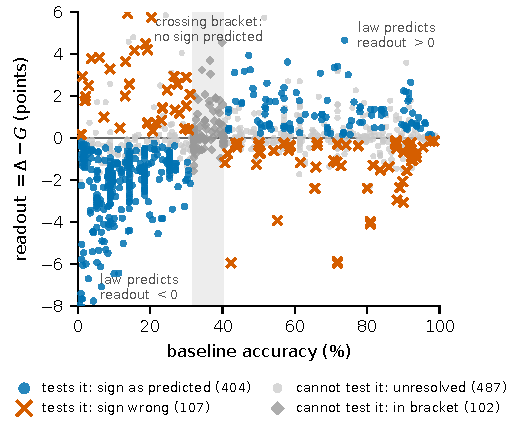
\includegraphics[width=\linewidth]{figs/law_scatter.pdf}
\caption{The law, in full: \readout{} $=\Delta-G$ against baseline accuracy
for all \auditScope{} law-scope cells with ${\geq}3$ seeds on both arms. Shaded
band: the measured crossing bracket $[31.8,40.3]$, inside which no sign
is predicted. Only the first two legend entries test the account: of the \auditResolvable{}
cells whose \readout{} is resolvable against its own seed-paired uncertainty,
\auditCorrect{} fall on the predicted side of zero. The other two entries keep the audit's reach visible:
\auditUnresolved{} are unresolvable and \auditBracket{} sit inside the
bracket, so the rate is $\auditRate\%$ at $\auditCoverage\%$ coverage against a
$\auditMajority\%$ majority-sign baseline.
The scatter at fixed baseline is substantial ($R^2 = 0.27$, residual SD
$\auditResidSD$ points): the account predicts the sign of this term, not its value.}
\label{fig:law}
\end{figure}

\looseness=-1 That regularity is not a theorem but an empirical one with measured scope,
registered in advance (Sec.~\ref{sec:lawpredict}) and found only after two
wrong intermediate laws, a ``deficit'' law and a multiplicative
realization$\times$gain form, were falsified by our own cells and retracted.
Its content is asymmetric: below the crossing it predicts a large negative
\readout{} and is strongly falsifiable; far above it predicts \readout{}
${\approx}0$, true but weakly discriminating, so a naive sign-count over
high-data cells would produce a coin flip and wrongly suggest failure. The
audit therefore counts only cells whose \readout{} is resolvable against its own
\emph{seed-paired} uncertainty (Sec.~\ref{sec:stats}), tighter than
independent propagation and the protocol the released script implements.

\subsection{The audit}\label{sec:lawaudit}
\begin{table}[pos=htbp]
\caption{Scope-wide sign-law audit, regenerated from the per-run records by the
released audit script. A cell is resolvable when $|\readout| > 2\,\mathrm{SEM}$; cells inside
the crossing bracket make no sign prediction. Uncertainty is seed-paired
(Sec.~\ref{sec:stats}), not propagated from independent arms. Scope is
aux-from-scratch: cells carrying an ImageNet or self-supervised
initialization are excluded here and scored separately in
Sec.~\ref{sec:fusion}, and $100\%$ cells report only the aux-vs-baseline
gap under the scope rule of Sec.~\ref{sec:probe}, which is why the
first row is much larger than the
second; the rows narrow to the resolvable subset that actually tests the
account.}
\label{tab:audit}
\centering\scriptsize
\setlength{\tabcolsep}{2.6pt}
\zebra{2}
\begin{tabular}{lr}
\toprule
Population & Cells \\
\midrule
Cells with paired $\Delta$ and $G$ (all interventions) & \auditAllPaired \\
\quad in scope, ${\geq}3$ seed-matched arms & \auditScope \\
Backbone variants in scope (architecture families) & 7 (5) \\
Dataset identities in scope & 20 \\
Inside crossing bracket (no prediction) & \auditBracket \\
Unresolved ($|\readout| \le 2$\,SEM) & \auditUnresolved \\
\midrule
\textbf{Resolvable (these test the account)} & \textbf{\auditResolvable} \\
\quad Sign as predicted & \textbf{\auditCorrect{} (\auditRate\%)} \\
\quad Wrong side & \auditWrong \\
\bottomrule
\end{tabular}
\end{table}

\begin{table}[pos=htbp]
\caption{Robustness of the audit: the rate is stable against the
resolvability threshold, survives clustering on the units that share a
baseline arm, and survives re-fitting the crossing bracket without the
audited dataset (the out-of-sample check). It is carried by
the left flank, where the account predicts strongly, not by the
right, where it predicts ${\approx}0$. Intervals are Wilson 95\%.}
\label{tab:robust}
\centering\scriptsize
\setlength{\tabcolsep}{2.6pt}
\zebra{2}
\begin{tabular}{P{0.30\columnwidth}rrrP{0.20\columnwidth}}
\toprule
Audit variant & Cells & Correct & Rate & 95\% CI \\
\midrule
$|\readout| > 1$\,SEM & 629 & 509 & 80.9\% & [77.7, 83.8] \\
$>1.5$\,SEM & 531 & 446 & 84.0\% & [80.6, 86.9] \\
\textbf{$>2$\,SEM (declared)} & \textbf{\auditResolvable} & \textbf{\auditCorrect} & \textbf{\auditRate\%} & \textbf{[82.9, 89.2]} \\
$>3$\,SEM & 342 & 304 & 88.9\% & [85.1, 91.8] \\
\midrule
One vote per (dataset, backbone, fraction) & 235 & 192 & 81.7\% & [76.3, 86.1] \\
Held out: bracket fitted without the audited dataset & 391 & 347 & 88.7\% & [85.2, 91.5] \\
\midrule
Below the crossing & 314 & 298 & 94.9\% & [91.9, 96.8] \\
Above the crossing & 141 & 95 & 67.4\% & [59.3, 74.6] \\
\bottomrule
\end{tabular}
\end{table}

\looseness=-1 Table~\ref{tab:audit} summarizes the audit: of \auditResolvable{} resolvable
cells spanning seven backbones and nineteen of the twenty dataset identities
in scope (the caption of Table~\ref{tab:partitions} explains why identities
outnumber image sources; one has law-scope cells but no resolvable one), \auditCorrect{}
($\auditRate\%$) fall on the predicted side (Wilson 95\% CI $[82.9, 89.2]$).
Eleven cells entered scope late, ten of them resolvable, when the
prior-with-augmentation arms of Sec.~\ref{sec:stack} and the fixed-step
cells acquired their frozen-feature evaluations. All
are aux-from-scratch cells with both measurements, so the law's own definition
admits them, excluding them after seeing their effect would be the
selection this benchmark exists to expose, and admitting them lowered the
rate by three-tenths of a point, on overlapping intervals.

\looseness=-1 Two numbers belong beside that one. The resolvability rule decides which
cells vote, and only $\auditCoverage\%$ of scope cells do, so we write the
result as $\auditRate\%$ \emph{at $\auditCoverage\%$ coverage} throughout.
The null matters as much: an exact binomial against a coin returns $p \approx
2\times10^{-58}$, true and useless, because nobody proposes a coin. The
\readout{} term is
negative in most resolvable cells, so always predicting negative already
scores $\auditMajority\%$; the account beats that, but the honest effect size
is the gap to $\auditMajority\%$, not to $50\%$. Below the crossing, where
the account makes a strong prediction, it is $298/314 = 94.9\%$; above it,
where it predicts only that the term is small, $95/141 = 67.4\%$. The
\auditWrong{} exceptions group rather than scatter. One carries a single
signature, $G$ clearly positive while $\Delta$ is negative at ${\geq}20\%$ data
on Food-101 and PathMNIST, ``better features, worse accuracy at sufficiency''.
A second is an artifact of the account's \emph{input}, not its prediction: the
two largest exceptions are Swin cells whose baseline arm is seed-bistable, so
their nominal baseline height averages trained and collapsed seeds and does not
measure how well the task is being solved. We leave them in the count and name
them instead: dropping bistable-baseline cells would raise the reported rate,
so excluding them is not a neutral choice. Table~\ref{tab:exceptions} lists the largest-magnitude exceptions
individually, because where an account fails is part of what it claims.

\paragraph{Two scope repairs that moved this number, and by how much.}
\looseness=-1 An earlier version of this audit reported $\auditPrevRate\%$
over $\auditPrevResolvable$ resolvable cells from a scope of
$\auditPrevScope$; the figure is higher because two scope filters were
repaired, not because any run, seed or measurement changed. First, cells
carrying an ImageNet initialization, the interference case of
Sec.~\ref{sec:taxsub} and outside the regime the \readout{} branch was
estimated in, leaked in through a string mismatch: the filter tested the
exported \texttt{pretrained} field against \texttt{true} and \texttt{1}
while the exporter writes \texttt{yes}. Restoring it removes
\auditExclCells{} cells, \auditExclResolvable{} of them resolvable
(\auditExclCorrect{} correct, \auditExclWrong{} wrong,
$\auditExclRate\%$ on their own), taking the scope to $\auditMidScope$
and the rate to $\auditMidRate\%$ over \auditMidResolvable{} resolvable
cells; below the
crossing the $298$ correct cells are untouched while $23$ wrong ones leave
($\auditPrevBelowRate\%$ to $\auditMidBelowRate\%$),
Sec.~\ref{sec:taxsub} seen from the other side. Second, at $100\%$ cells
Sec.~\ref{sec:probe} reports the aux-vs-baseline gap and refuses the
$G$/\readout{} split, yet the released script carried no such filter.
Removing the \auditHundredCells{} full-data cells drops
\auditHundredResolvable{} resolvable cells (\auditHundredCorrect{} correct,
\auditHundredWrong{} wrong, $\auditHundredRate\%$ on their own, the
worst-scoring subset in the audit and exactly the cells the rule calls
uninterpretable), moving the headline from $\auditMidRate\%$ to
$\auditRate\%$ and the below-crossing flank to $\auditBelowRate\%$
(\auditHundredBelow{} more cells, both wrong). The price is breadth: ViT-S,
ViT-B and ImageNet-100 hold law-scope cells only at $100\%$, so the span
narrows from nine backbones to seven and from twenty-one dataset identities
to twenty, though the five architecture families survive. Both pre-repair
headlines and both excluded subsets' own rates are stated above so the
repair stays visible. Sec.~\ref{sec:scale} is untouched:
Table~\ref{tab:scale} reports $\Delta$, $G$ and their gap with no signed
\readout{}, which the rule permits, so the ImageNet $\Delta \approx G$
result stands while the same cells leave the sign-law count.

\begin{table}[pos=htbp]
\caption{The ten largest-magnitude resolvable exceptions, of
\auditWrong{} in total, printed from the same audit as
Table~\ref{tab:audit}; they cluster, not scatter. \emph{Top:} Swin cells
whose baseline arm is unstable (seed SD $10$--$22$ points), so the baseline
height the account takes as input is not a task-performance reading; the
records flag the first two as bistable and the third narrowly not.
\emph{Second:} the ``better features, worse accuracy at sufficiency''
signature. \emph{Third:} PathMNIST, whose linear evaluation is a compressed
measuring stick. \emph{Bottom:} two heavily-augmented ViT cells on DTD, with
\readout{} positive far below the crossing.}
\label{tab:exceptions}
\centering\scriptsize
% 8 columns = 16 gutters, so each 0.1pt here is 1.6pt of width. At 2.6pt this
% ran 3.01pt over the measure. Narrowing the gutter also shrinks the zebra
% overhang, which is \tabcolsep on each side, so it stays inside the rules.
\setlength{\tabcolsep}{2.3pt}
\zebra{2}
\begin{tabular}{lllrrrrr}
\toprule
Dataset & Backbone & Variant & Frac. & Base & $\Delta$ & $G$ & \textit{Readout} \\
\midrule
EuroSAT & Swin & aux & 20\% & 22.7 & $+71.27$ & $+55.93$ & $+15.34$ \\
EuroSAT & Swin & aux & 15\% & 18.6 & $+73.72$ & $+61.66$ & $+12.06$ \\
EuroSAT & Swin & aux & 2\%  & 42.3 & $+30.54$ & $+36.49$ & $-5.95$ \\
\midrule
Food-101 & R18 & mag3 & 50\% & 71.8 & $-1.30$ & $+4.66$ & $-5.96$ \\
Food-101 & R18 & mag6o & 50\% & 71.8 & $-0.91$ & $+4.97$ & $-5.88$ \\
Food-101 & MNet & aux & 50\% & 55.1 & $-0.23$ & $+3.70$ & $-3.93$ \\
\midrule
PathMNIST & R18 & mag6o & 1\% & 80.8 & $+5.80$ & $+9.90$ & $-4.09$ \\
PathMNIST & R18 & mag3 & 1\% & 80.8 & $+5.62$ & $+9.60$ & $-3.98$ \\
\midrule
DTD & ViT & deit-aux & 100\% & 13.2 & $+25.55$ & $+21.91$ & $+3.63$ \\
DTD & ViT & deit-aux & 50\% & 14.2 & $+17.30$ & $+14.73$ & $+2.57$ \\
\bottomrule
\end{tabular}
\end{table}

Table~\ref{tab:robust} reports what that number survives. Not the resolvability
threshold: the rate moves only from $80.9\%$ over 629 cells at one SEM to
$88.9\%$ over 342 at three, so a stricter or looser criterion reaches the same
conclusion. Not the dependence between cells: collapsing to one vote per
(dataset, backbone, fraction) leaves $192/235 = 81.7\%$. And, the check that
matters most, not the estimation of the crossing bracket on the cells we then
audit: re-fitting it on the other datasets and auditing each dataset out of
sample gives $347/391 = 88.7\%$, indistinguishable from the in-sample figure.

That row audits 391 cells, not all \auditResolvable{}, and the shortfall is not
a sampling choice. Re-fitting the bracket on the other datasets widens it
beyond the pooled $[31.8, 40.3]$, since one dataset's cells no longer pin
either edge (for CIFAR-100 it becomes $[29.5, 71.0]$), and cells inside a
bracket make no sign prediction, so $46$ leave the held-out set that way, 25 of
them CIFAR-100's; a further $18$ sit in datasets that cannot receive a fold
($391 + 46 + 18 = \auditResolvable$). The bias runs one way: the held-out row
keeps the cells furthest from the crossing, where the account is most
confident, so its rate is a mild upper bound rather than a like-for-like
comparison, and the effect is small since $86\%$ of resolvable cells do receive
an out-of-sample verdict.

What the number does \emph{not} survive is disaggregation. The evidence is
overwhelmingly left-flank: below the crossing the sign is right $94.9\%$ of the
time, above it $67.4\%$, close to a coin once the term it predicts has shrunk
to nothing. One dataset behaves badly out of sample, PathMNIST at $52.6\%$: its
linear evaluation is a known compressed measuring stick, its frozen-feature
accuracy sitting \emph{below} its own end-to-end accuracy, so we treat its
$G$ as unreliable there, not the account as refuted, and report the failure
instead of excluding the dataset. We do not explain this cluster; we name it
as the law's known boundary (Sec.~\ref{sec:limits}), and the released audit
script enumerates every exception.

\paragraph{What the \readout{} term is, once the label budget is matched.} Every
$G$ above uses one evaluation budget for all cells, the full training split,
while the cell itself trained on a fraction of it: at $1\%$ the evaluation
holds a hundred times the cell's labels. That asymmetry could on its own
explain the negative branch, so we measured it, re-evaluating both arms of $30$
reference-configuration cells across seven datasets, baselines $5.3$ to $93.8$, at \emph{each
cell's own} per-class budget (five to $2{,}500$ labels per class).

The stronger result comes first. At matched budget the end-to-end gain and the
frozen-feature gain agree to $0.17$ points on average, median $0.11$ and worst
case $0.77$, against $0.89$ under the full-label protocol. A linear evaluation
run at the label budget a practitioner actually has therefore predicts the
end-to-end difference between two arms without training either combination, and
what had been a two-cell observation now holds over $30$ cells and seven
datasets.

The second result follows from it and cuts against our own framing, which is
why we registered it in advance. The \readout{} term largely disappears at matched
budget: below the crossing its mean moves from $-1.66$ to $-0.19$ and above it
from $+0.10$ to $-0.13$, $19$ of $30$ cells lose more than half their
magnitude, and only $3$ of $30$ stay resolvable against their own uncertainty.
Below the crossing the negative sign is thus substantially a statement about
the ratio of evaluation labels to training labels, for which baseline accuracy
is a monotone proxy, rather than an independent property of training. The sign
law remains an accurate description of the full-label protocol, the protocol
every $G$ in this paper is measured under, so Tables~\ref{tab:audit} and
\ref{tab:robust} stand exactly as measured; what changes is how to read them.

\subsection{Prediction, not description}\label{sec:lawpredict}
Three pre-registered episodes distinguish the law from a post-hoc fit.

\emph{(i) A new backbone family from baselines alone.} Before any Swin-T linear
evaluation existed, we read the \readout{} term off the measured curve at Swin's
baseline heights and published bands for its feature gain ($G \approx 9.6$,
$8.8$, $9.8$ and $7.0$ at 5, 10, 15 and 25\% of CIFAR-100; band $+7$--$+11$).
The measurements landed at $10.5$, $9.3$, $10.1$, $7.6$: four of four in band,
each within one point of its point call, against two live falsifiers
(attention-intrinsic $G{\geq}13$; stabilization-only $G{\leq}6$), either of
which would have refuted the account.

\emph{(ii) Four unseen domains.} The same procedure applied to satellite,
texture, food and histopathology cells straddling the crossing produced eight
banded predictions; seven landed in band and all eight had the predicted sign,
including the two deliberately hard cases where a small $\Delta$ could have
hidden a large $G$ (it did not: small $\Delta$ meant small $G$).

\emph{(iii) ImageNet scale}, the subject of Sec.~\ref{sec:scale}, where the
residual $\Delta - G$ was pre-registered to stay within $1.5$ points on every
backbone.

\subsection{What $G$ is a function of}\label{sec:lawG}
Controlled crossings localize the law's terms. $G$ is a property of the
checkpoint and the evaluation's label space. It is invariant to which coarse
partition relabels the data, but is cut roughly from $4.2$ to $2.9$ when
training supervision moves from 200-way fine to 20-way coarse labels on
identical pixels: fine-grained weak supervision is where the prior has the most
feature work to do. The \readout{} term follows task performance, not label
budget: engineered cells that lower class count without raising baseline
accuracy get no \readout{} boost (a prediction our own account initially got
wrong, and the cell that corrected it is in \ref{app:controls}). And
$G$ depends on the backbone as sharply as on the data: at the same
Tiny-ImageNet cell, ResNet-18 carries $G = +2.66$ while MobileNetV3 carries $G
= +0.01 \pm 0.23$, a measured zero on the weaker network, so ``how much a prior
can add'' is not a dataset property but a (dataset, architecture) property.

\subsection{What the prior leaves behind}\label{sec:imprint}
\begin{figure}[pos=htbp]
\centering
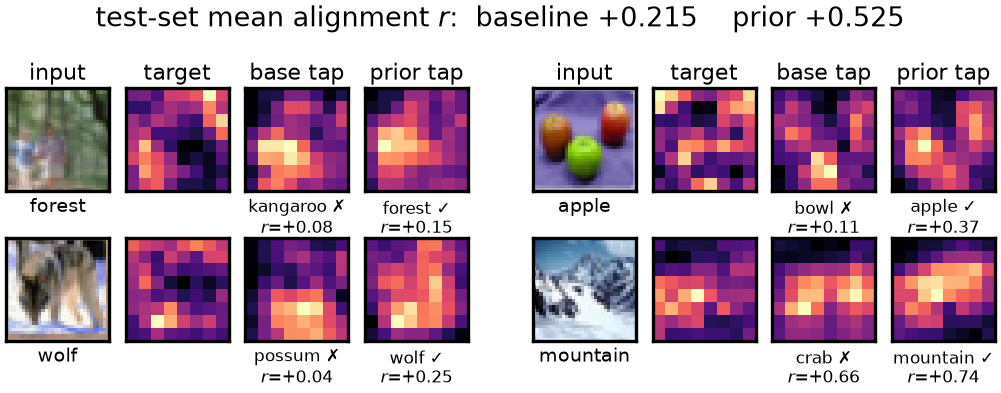
\includegraphics[width=\linewidth]{figs_explain/heatmaps_auxmag_5pct_sched0.png}
\caption{The spectral imprint at the tap, CIFAR-100 at 5\%. Columns:
input, the fixed moment target, and the tapped-stage energy of the
baseline and prior arms. Over the \emph{whole} test set the alignment
between tapped features and the target is $+0.215$ for the baseline and
$+0.525$ for the prior arm. The three rows are \emph{selected} cases
(prior arm correct, baseline wrong), so they illustrate the alignment
difference, not sample it, and only the test-set-wide figure
should be read as evidence.}
\label{fig:heatmap}
\end{figure}
$G$ is a number, and it is worth seeing what in the representation it
corresponds to. The prior's target is a fixed bank (Fig.~\ref{fig:bank}), and
its imprint survives to the end of training: at the CIFAR-100 5\% cell, where
the feature gap is largest on this dataset ($+6.3$ points), the alignment
between tapped features and the bank's oriented-energy target measured over the
whole test set is $+0.525$ for the prior arm against $+0.215$ for the baseline
(Fig.~\ref{fig:heatmap}). That it survives is the part that matters, because the auxiliary weight
decays to exactly zero well before training ends: the prior changes where the
representation settles, not what the loss pulls on at the finish.

\begin{figure}[pos=htbp]
\centering

\includegraphics[width=\linewidth]{figs_explain/cam_auxmag_5pct_sched0.png}
\caption{Where the class evidence sits, CIFAR-100 at $5\%$. The three rows are
\emph{selected} cases (prior arm correct, baseline wrong), so they show what the
difference looks like where it is present, not how often. The evidential
quantity is measured over the whole test set instead: the Gini coefficient of
each class-activation map normalized to sum one, where higher means evidence
concentrated at fewer locations, gives $\camBase$ for the baseline against
$\camAux$ for the prior arm over $\camN$ images ($\camSigma\,\sigma$). The
prior's evidence is measurably more
concentrated, by a modest amount, not the categorical difference the three
rows suggest.}
\label{fig:cam}
\end{figure}

A second, independent read asks not what the features encode but where the
class evidence sits: Fig.~\ref{fig:cam} scores the concentration of each
class-activation map over the whole test set, and the prior's evidence is
measurably more concentrated, though only by $+\camDelta$.

\paragraph{Is that imprint specific, or is it what good features look like?}
One cell cannot tell the two apart, and any intervention that improves features
might show the same alignment, so we measured the same statistic across
families that reach a positive $G$ by \emph{different} routes, against one
pinned target for every model, since a self-supervised initialization has no
auxiliary head and therefore no target of its own. Reporting the alignment gap,
each arm minus its own baseline (Table~\ref{tab:imprint},
Fig.~\ref{fig:imprint2}):

\begin{table}[pos=htbp]
\caption{The imprint follows the \emph{target}, not the feature gain.
Alignment gap is the arm minus its own baseline, CIFAR-100/ResNet-18, one
pinned target applied to every model. The lower block is a $2\times2$ that
fell out of the design: crossing \{self-supervised initialization or not\}
with \{moment target or not\}, the imprint tracks the target while $G$
tracks the initialization. Best in bold, second best underlined, third best
in italics, per numeric column; the two columns' markings disagree.}
\label{tab:imprint}
\centering\scriptsize
\setlength{\tabcolsep}{4pt}
\zebra{2}
\begin{tabular}{lrrr}
\toprule
Family & $n$ & mean $G$ & alignment gap \\
\midrule
Moment prior (tap L3)        & \imprintPriorN & $+\imprintPriorG$ & \snd{$+\imprintPrior$} \\
SimCLR init, no target       & \imprintSSLN   & \snd{$+\imprintSSLG$}   & $\imprintSSL$ \\
Random fixed target          & 1              & $+1.31$           & \trd{\imprintRand} \\
\midrule
Moment prior, tapped at L1/L2 & 2 & \trd{+4.67} & $\imprintTap$ \\
SimCLR init $+$ moment target & 1 & $\mathbf{+8.08}$ & $\mathbf{+\imprintCombo}$ \\
\bottomrule
\end{tabular}
\end{table}

\begin{figure}[pos=htbp]
\centering
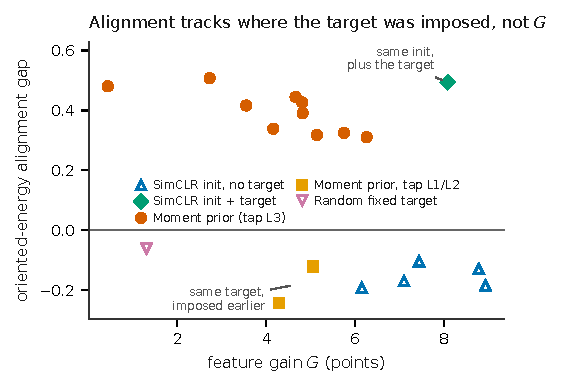
\includegraphics[width=\linewidth]{figs/imprint_dissociation.pdf}
\caption{Alignment gap against feature gain, one point per cell, CIFAR-100 /
ResNet-18. Filled markers had the moment target during training. The two
quantities are independent: every cell whose target was imposed at the tapped
stage sits at $+0.31$ to $+0.51$ regardless of whether its $G$ is $2.7$ or
$8.1$, and every cell without a target there sits below zero across the same
range of $G$. The two labelled controls separate the accounts: the
same target imposed two stages earlier leaves no imprint at layer~3, and the
same self-supervised initialization as the negative points, with the target
added, gives the largest gap measured.}
\label{fig:imprint2}
\end{figure}

The self-supervised cells are the decisive comparison and they answer it in the
strongest available direction: they carry \emph{more} feature gain than the
prior ($G = +\imprintSSLG$ against $+\imprintPriorG$) and \emph{less}
oriented-energy structure than their own baselines ($\imprintSSL$). We had
registered a band of $-0.05$ to $+0.10$ for them and a falsifier at $\geq
+0.15$; the measurement came back at the opposite sign, so oriented-energy
alignment is not simply what better features look like on this data.

Two controls fell out of the design unplanned, and each isolates one factor
more sharply than the comparison we set out to make. Moment-prior cells
\emph{tapped two stages earlier} use the identical target and show
$\imprintTap$ when read at layer~3: the imprint is localised to where the
target is imposed, which a mechanism predicts and an incidental correlation
does not. And a cell with the same SimCLR initialization as the $\imprintSSL$
rows, plus the moment target, shows $+\imprintCombo$, the largest gap we
measure. Crossed, these give a $2\times2$ in which the imprint follows the
target and $G$ follows the initialization.

What this does \emph{not} establish: alignment is a correlation between
channel-\emph{mean} energy maps, so it measures agreement in spatial layout,
not reproduction of the individual oriented channels, and a null on it would
not rule out a finer imprint. The two control rows are single cells.

\begin{figure}[pos=htbp]
\centering
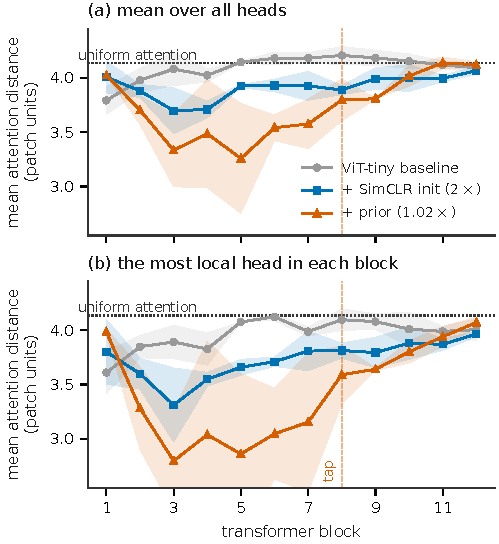
\includegraphics[width=\linewidth]{figs/attention_locality.pdf}
\caption{What the prior gives a small transformer: locality. Mean
attention distance per block, ViT-tiny on CIFAR-100 at 10\%, three seeds
(band: $\pm$1 SD). The dotted line is the distance a \emph{uniform} attention
map would give on this $8\times8$ token grid ($4.14$ patch units), computed, not assumed. The baseline sits on that line at every depth, never
learning to attend locally from 5{,}000 images; the prior
pulls the middle blocks well below it, most sharply \emph{upstream} of the
tap. A SimCLR initialization at $2\times$
the compute does the same, more weakly.}
\label{fig:attention}
\end{figure}
The same question can be put to the backbone where the prior matters most,
and there the answer is unusually legible. A vision transformer has no
built-in notion that nearby patches belong together; the standard diagnostic
for whether it has learned one is mean attention distance.
Figure~\ref{fig:attention} measures it for ViT-tiny at CIFAR-100 10\%: the
baseline's heads straddle the uniform-attention distance at every depth, never
discovering locality on 5{,}000 images, while the prior pulls the middle
blocks well below it. The prior does not merely improve the features; it
supplies the spatial inductive bias the architecture lacks, which a
convolutional backbone gets for free and is why the same intervention is worth
several times more here.

We had predicted this effect in the \emph{early} blocks, decaying with depth,
and that is not what happened: at block~1 the ordering is nominally reversed,
the effect peaks at blocks~3--7, and the curves rejoin by block~11. The
location is interpretable after the fact, since the target is regressed from
block~8 and the locality appears in the blocks that feed it, but we did not
predict it and record it as a missed call on a held prediction, not a
confirmation. A SimCLR initialization produces the same signature at about half
the depth-integrated magnitude, which is consistent with the two being
substitutes on this backbone.

We are deliberate about how far the qualitative evidence goes. The
individual-image maps of Figs.~\ref{fig:heatmap} and \ref{fig:cam} are
selected on cases the prior gets right
and the baseline wrong, so they illustrate rather than demonstrate; a t-SNE
of the frozen features (Fig.~\ref{fig:tsne}) moves the all-class silhouette
only from $-0.072$ to $-0.064$, since a $+6.3$-point feature gap need not be
legible in two projected dimensions. The alignment statistic and the linear
evaluation are the measurements; the pictures illustrate them.

%% ---------------------------------------------------------------------
\section{Fusion outcomes: stack, substitute, interfere}\label{sec:fusion}

The grid's central comparative finding is that fusion outcomes are predictable
from the \emph{currency} each information source supplies.

\textbf{What we mean by currency, operationally.} The word is a metaphor
used once as one; what it stands for is a measurement from single-source
quantities only, so nothing in it requires training the combination. A
source's currency is characterised from that source \emph{alone}: the
frozen-feature gain $G$ it produces under the declared protocol, together
with \emph{what} it improves, that is, which test images its arm fixes and
how similar its learned representation is to the other source's, both
measured on the single-source arms (Sec.~\ref{sec:samecurrency}). Two
sources trade in the same currency when, at a matched cell, their $G$ values
agree \emph{and} their single-source arms agree, on images fixed and in
representation, about as closely as two seeds of one source do; both halves
are necessary because two representations can raise linear accuracy equally
while encoding different things. The combination's $G$ appears nowhere in
the definition; it is what the definition \emph{predicts}, same currency
implying that the combination's $G$ will not exceed the better single
source, and Secs.~\ref{sec:substitute} and~\ref{sec:samecurrency} test
that prediction. $G$ is a cheap ordinal proxy for source overlap, not an
estimate of the unique and redundant atoms that partial information
decomposition formalizes (Sec.~\ref{sec:fusiontheory}); what it buys is
measurability on each source alone, at the cost of one linear fit, which is
what makes a prospective rule possible at this grid's scale.

This section presents the three outcomes in order of how favorable they are:
different currencies can compound, differing currency being necessary while
architecture and intervention strength decide how much is realized
(Sec.~\ref{sec:stack}); the
same currency
adds nothing, with the refinement that rescues the rule from its apparent
counterexamples (Sec.~\ref{sec:substitute}); and one fusion, at full
shaping strength, is uniformly
destructive, with the feature-level measurement that explains why
(Sec.~\ref{sec:taxsub}). Section~\ref{sec:taxonomy} collects the three
into a single table with the evidence for each row.

\subsection{Different currencies can stack}\label{sec:stack}
DeiT-strength augmentation supplies invariance to nuisance transforms; the
prior supplies oriented-energy structure. Fusing both
(Table~\ref{tab:vitenvelope}) does not trade off: the prior's ViT gain grows
under augmentation on both populations, by $1.5$--$2.4\times$ on CIFAR-100 and
$1.4$--$2.4\times$ on Tiny-ImageNet across $1$--$25\%$. We give the two ranges
separately because we once gave one: a registered ``$1.8$--$2.4\times$
throughout'' missed low on Tiny-ImageNet at 5, 15 and $25\%$, so amplification
is population-dependent and the CIFAR-100 range was over-generalized. On
Tiny-ImageNet it also vanishes at full data ($0.92\times$), where both
interventions are decaying anyway. The feature side confirms the mechanism: the prior's $G$
\emph{rises} under augmentation (from $14.8$ to $22.2$ at 10\%), because once
nuisance variation is handled the network can commit more capacity to the
structure the target teaches. Our own pre-registered bet here was wrong in the
pessimistic direction: we predicted partial substitution and measured strong
complementarity.

\paragraph{How far that reaches, on a convolutional backbone.} Every cell
above is a ViT, on CIFAR-100 (the selection set) or Tiny-ImageNet (no part in
selection, Sec.~\ref{sec:selection}). What the result does not span is a
convolutional backbone off the selection set, so we ran the three missing
fusion arms there, augmentation alone, prior with augmentation, and prior
with a SimCLR initialization, on EuroSAT and Food-101 with ResNet-18 at 5, 10
and $25\%$. The substitution result transplants; the stacking result does
not.

\looseness=-1 Prior with SimCLR falls below the better single source at all six cells
($-0.14$ to $-2.41$), so on these convolutional populations it does not merely
fail to add, it costs, and the registered falsifier for the substitution rule,
a combination beating the better single by ${\geq}1.5$, fired nowhere. Prior
with augmentation stacks at exactly one cell of six, Food-101 at $5\%$
($+4.32$, eleven standard errors), and is negative at the other five ($-0.37$
to $-3.07$). That tripwire required failure on \emph{both} populations, so it
did not fire on the letter; we report it as a narrowing rather than a pass.
Prior-with-augmentation stacking is therefore a result about attention
backbones, holding on both the selection population and an off-selection one,
plus a single convolutional cell; it is not a general property of the two
currencies.

\looseness=-1 What does hold across these cells and the schedule control of
Sec.~\ref{sec:taxsub} concerns strength. Adding the prior at full weight
costs whenever the partner is already strong: where augmentation is harmful the
prior leads (EuroSAT at $5\%$, augmentation alone $-7.67$ against the prior's
$+0.84$), and where augmentation is strong the prior subtracts (Food-101 at
$10\%$, augmentation alone $+9.26$, adding the prior $-1.81$). Frozen-feature
evaluation of the same arms agrees: measured against the same partner alone,
the prior moves $G$ by $+4.68$, $-1.22$ and $-1.51$ on Food-101 over
augmentation at 5, 10 and $25\%$, and by $-1.38$, $-2.29$ and $-1.27$ over the
SimCLR initialization, so the cost is feature-side here as for the transfer
tax. One more thing the attention-only evidence had hidden: DeiT-strength
augmentation is not universally good, worth $+9.45$, $+9.26$ and $+3.05$ alone
on Food-101 but $-7.67$, $-0.14$ and $+0.11$ on EuroSAT, so a claim about
augmentation as a fusion source has to name its domain.

\subsection{Same currency substitutes}\label{sec:substitute}
\begin{table}[pos=htbp]
\caption{Prior versus SimCLR initialization ($2\times$ compute) on
ViT-tiny, CIFAR-100, and the effect of recipe. Under plain augmentation
SSL catches the prior at ${\sim}5$k images; under the DeiT recipe the
prior wins at every fraction because the recipe supplies the invariance
SSL was selling. Three seeds per cell, six on the DeiT-recipe $5\%$ arm. A positive entry is a fraction
where the prior wins; no better-direction marker is used, since neither
sign of a method-versus-method difference is better a priori. Per fraction
the recipe under which the prior stands better is bold; with two rows the
second-best and third-best marks do not apply.}
\label{tab:flip}
\centering\scriptsize
\setlength{\tabcolsep}{2.6pt}
\zebra{4}
\begin{tabular}{lrrrrr}
\toprule
 & \multicolumn{5}{c}{prior $-$ SimCLR (points)} \\
\cmidrule(l){2-6}
Recipe & 1\% & 5\% & 10\% & 25\% & 100\% \\
\midrule
Plain crop+flip & $+0.7$ & $+1.3$ & $0.0$ & $-1.4$ & $-3.9$ \\
DeiT augmentation & $\mathbf{+2.5}$ & $\mathbf{+7.2}$ & $\mathbf{+5.2}$ & $\mathbf{+5.0}$ & $\mathbf{+2.0}$ \\
\bottomrule
\end{tabular}
\end{table}

\looseness=-1 SimCLR's objective \emph{is} invariance to an augmentation family. Three
measurements pin the consequence. First, prior and SimCLR never stack: on
convolutional backbones the combination costs $-1.5$ points against SimCLR
alone, and on ViT it is exactly neutral against the better single arm. Their
feature gains are the same gain ($G = 14.8$ against $13.5$ at the same cell),
so the second source has nothing left to add. Second, the head-to-head flips
with the recipe (Table~\ref{tab:flip}): under plain augmentation SSL overtakes
the prior once data is plentiful, but under the DeiT recipe, the recipe anyone
training a small ViT would actually use, the prior wins at every CIFAR-100
fraction, by ${\sim}5$ points across the mid-band, and the feature side shows
why: augmentation lifts the prior's $G$ by $+7.4$ but SimCLR's by only $+3.8$
at 10\%. The same flip reproduces on Tiny-ImageNet in the low-data band. Third,
SimCLR was not under-equipped: giving its contrastive views DeiT strength makes
it \emph{worse} at every fraction (by $4$--$12$ points e2e, halving its $G$),
so its standard configuration was its strongest available one.

The substitution rule refines rather than universalizes: fusing the prior onto
\emph{ineffective} SSL stacks trivially. SimSiam at its published
budget learns almost nothing at study scale ($\Delta \leq +0.9$ at every
CIFAR-100 and CIFAR-10 fraction, ${\leq}+1.8$ on any population), and
prior-on-SimSiam recovers the prior's full gain ($+6.2$ and $+4.3$ over
SimSiam alone at CIFAR-100 5 and 10\%, and $+2.0$ at Tiny-ImageNet 5\%). The operative rule is therefore \emph{the prior is
redundant exactly insofar as the other source already bought the same
features}, judged by the other source's own measured gain, not by its family
name.

\looseness=-1 The grid contains the intermediate case, and it contradicts the binary phrasing
of Table~\ref{tab:taxonomy}'s second row while supporting the rule just stated.
On ViT-tiny at CIFAR-100, prior with a DINO initialization beats the better
single arm by $+0.92$ at $10\%$ ($30.66$ against the prior's $29.74$, about
five standard errors) and $+1.02$ at $5\%$ ($22.62$ against $21.60$), and a
combination exceeding both singles is what that row says cannot happen. The
refined rule predicts it: DINO is a partial source here, its feature gain
$+7.90$ roughly half the prior's $+14.83$, so it has not bought the same
features and work is left for the prior to do. The feature side confirms rather
than merely permits that reading, since the combination's $G$ is $+14.77$,
level with the prior alone, not above it: the two still substitute in
feature space even as the combination edges ahead end to end. We therefore state the row as \emph{combination $\leq$ best
single when the partner's $G$ matches the prior's, and partial when it does
not}, and we count these cells as the case that forced the qualification.

\subsection{Fusing into mature features interferes}\label{sec:taxsub}
\begin{table}[pos=htbp]
\caption{The interference tax of the ImageNet-transfer fusion, and its
feature-side origin. Injecting the
prior on top of ImageNet weights \emph{at full auxiliary strength} is
destructive in proportion to what the initialization supplied; linear
evaluation shows the loss is carried almost entirely by $G$ (features), not by
the \readout. PathMNIST, where ImageNet features barely transfer, is the null
control. Ten seeds on the two CIFAR pairs end-to-end, three on PathMNIST, and
three for every linear evaluation, so the \readout{} column differences a
ten-seed $\Delta$ against a three-seed $G$. The text below reports the same
three cells at reduced $\lambda_0$, where the tax disappears.}
\label{tab:tax}
\centering\scriptsize
\setlength{\tabcolsep}{2.6pt}
\zebra{2}
\begin{tabular}{lrrrrr}
\toprule
Dataset & Frac. & Transfer adv. & $\Delta$ (tax)~\up & $G$~\up & \textit{Readout} \\
\midrule
CIFAR-10 & 5\% & $+9..{+}14$ & $-15.2$ & $-15.8 \pm 1.7$ & $+0.6$ \\
CIFAR-100 & 7\% & $+10..{+}18$ & $-16.8$ & $-16.3 \pm 3.1$ & $-0.6$ \\
PathMNIST & 10\% & $+1.8..{+}2.9$ & $-0.4$ & $+0.3 \pm 0.6$ & $-0.7$ \\
\bottomrule
\end{tabular}
\end{table}

The one uniformly destructive fusion in the grid is instructive
(Table~\ref{tab:tax}). The prior's early shaping at full strength, so valuable
from scratch, \emph{erases} mature ImageNet features. We call the measured
degradation an \emph{interference tax}, and the tax runs $-15.2$ to
$-16.8$ on the two datasets where
transfer was worth $+10$ to $+18$ on the cells of Table~\ref{tab:tax}, decays
to zero at full data (where the initialization no longer carries the
performance), and, the decisive measurement, lands almost entirely on $G$.
Where the initialization had little to offer (histopathology), there is nothing
to destroy and the tax is a measured zero. Fusion with an information-rich
partner must respect what the partner already encodes; a shaping prior does
not.

Table~\ref{tab:tax} shows the three cells we could also probe, and three cells
cannot carry a claim about a regime, so we state the population they come from:
of the \taxCells{} transfer cells that carry the prior \emph{at full auxiliary
strength from the first step} ($\lambda_0 = 1.0$, no delayed onset) at three or
more seeds, \taxNegative{} have a
negative $\Delta$, spanning nine datasets, with a median of $\taxMedian$ and a
worst case of $\taxWorst$. Not one is positive.

Full strength defines that population rather than describing it, so the
released records hold more aux-on-pretrained cells than the figure counts: the
reduced-strength and delayed arms below are the \emph{control} for this claim,
and counting them inside the population they exist to explain would remove the
``not one is positive'' by construction while establishing nothing. What the
\taxCells{} cells establish is that \emph{this} shaping schedule interferes, in
proportion to what the initialization supplied, and not that a structural prior
interferes with mature representations however it is applied.

\paragraph{The tax is a property of the schedule, not of the fusion.} We ran
that control on the three cells of Table~\ref{tab:tax} at $\lambda_0 = 0.3$,
$0.1$ and $0.05$, plus a delayed arm holding the prior at zero for the first
half of training, ten seeds per arm against ten-seed baselines on the two
CIFAR cells and three on PathMNIST. The
registered falsifier was that any arm reaching $\Delta \geq +0.5$ would show
the tax to be schedule-dependent, and two of the four CIFAR-100 arms clear it.

\looseness=-1 The tax does not scale smoothly with $\lambda_0$; it essentially vanishes below
full strength. On CIFAR-10 at $5\%$, $-15.2$ becomes $-0.18$, $+0.20$ and
$+0.05$ at $\lambda_0 = 0.3$, $0.1$ and $0.05$; on CIFAR-100 at $7\%$, $-16.8$
becomes $+1.50$, $+0.53$ and $+0.21$. The two halves carry different weight:
the disappearance is overwhelming, a $15$- to $18$-point move on both datasets,
while the CIFAR-100 arms coming out nominally \emph{positive} is not
established, pooling to $+0.70 \pm 0.61$, $1.1$ standard errors from zero, so
we do not claim the prior helps a pretrained initialization. Deepening from three seeds to ten shrank six
of the eight arms toward zero, every CIFAR-100 arm among them, the regression
to the mean Sec.~\ref{sec:stats} warns about, on our own result. PathMNIST, where the initialization had
nothing to supply, is unchanged across every arm
($-0.52$ to $+0.07$), as the currency account requires. The practical rule is
therefore not ``never'' but ``not at full strength'': at $\lambda_0 \leq 0.3$
the fusion is neutral on the cells we tested.

One prediction inside this control failed, and it bounds the mechanism. We
expected the delayed arm between $\lambda_0 = 0.3$ and $0.1$, on the account
that the damage is done in the early high-rate phase. It is instead the worst
arm below full strength on both datasets and negative on both, $-1.29$ on
CIFAR-10 at $6.3$ standard errors (the one clearly resolved cell here) and
$-0.31$ on CIFAR-100: withholding the prior and then applying
it at full weight is worse than applying a weak one throughout, so timing is
not the whole account and strength matters independently of it.

\subsection{The taxonomy}\label{sec:taxonomy}
\begin{table}[pos=htbp]
\caption{The fusion taxonomy the grid supports, with the measurement that
establishes each row. The rule's call uses only single-source measurements,
the two sources' frozen-feature
gains and what each improves, and the measured outcome matches it in all five
rows. Only the Sec.~\ref{sec:procedure} case was called before training, so
this is a taxonomy the rule organizes, not a prospective scoreboard. Each row
is scoped to the evidence beside it, and the first row is the narrowest: on two
convolutional populations outside the selection set the same pairing stacks at
one cell of six and mildly interferes at the rest
(Sec.~\ref{sec:stack}).}
\label{tab:taxonomy}
\centering\scriptsize
\setlength{\tabcolsep}{2.6pt}
\zebra{2}
\begin{tabular}{P{0.195\columnwidth}P{0.205\columnwidth}llP{0.225\columnwidth}}
\toprule
Fusion & Currencies & Call & Measured & Key evidence \\
\midrule
Prior + augmentation & structure + invariance & stack & \textbf{stack} & $\Delta$ amplified $1.4$--$2.4\times$ (1--25\%); $G\uparrow$ (ViTs; 1 of 6 conv cells off-selection) \\
Prior + effective SSL & structure $\approx$ invariance$^{*}$ & substitute & \textbf{substitute} & combo $\leq$ best single when $G$ matches; partial when it does not \\
Prior + ineffective SSL & structure + ${\sim}$nothing & stack & \textbf{stack} & full gain recovered on SimSiam \\
Prior + ImageNet init & structure vs.\ mature features & interfere & \textbf{interfere} & $-15$ to $-17$ e2e at $\lambda_0{=}1.0$, carried by $G$; null on shift; gone at $\lambda_0{\leq}0.3$ \\
Augmentation + SSL & invariance + invariance & substitute & \textbf{substitute} & DeiT recipe collapses SimCLR's margin \\
\bottomrule
\rowcolor{white}\multicolumn{5}{@{}p{0.95\linewidth}@{}}{\footnotesize $^{*}$Same
currency in effect: at matched cells the two sources' feature gains
coincide, which is why neither adds to the other.} \\
\end{tabular}
\end{table}

Table~\ref{tab:taxonomy} states the taxonomy compactly. Its practical force is
that the fusion outcome follows from quantities measurable before the
combination is trained: measure (or
look up) what each source contributes at the feature level, and same-currency
pairs will not add, while different-currency pairs can, when the strength and
the architecture cooperate (Sec.~\ref{sec:stack}).

\subsection{Same currency, same images}\label{sec:samecurrency}
Everything above infers currency from the \emph{magnitude} of a source's
feature gain. That is indirect: two sources could each add fourteen points
while improving entirely different images, and calling them the same currency
would then be an artifact of comparing scalars. We tested it directly, with the
prediction recorded first. Take three interventions on one backbone, dataset
and baseline (ViT-tiny, CIFAR-100 at 10\%): the prior, a SimCLR
initialization, and DeiT-strength augmentation. The taxonomy calls the first
two the same currency (they tie end to end, their feature gains are close, and
their combination is neutral) and the prior and augmentation different ones
(they stack), so the first pair should fix the same test images and learn more
similar representations than the second. Because easy images are fixed by
everything, we normalize each cross-intervention agreement by that
intervention's own agreement across seeds, the most same-currency comparison
available.

\begin{figure}[pos=htbp]
\centering
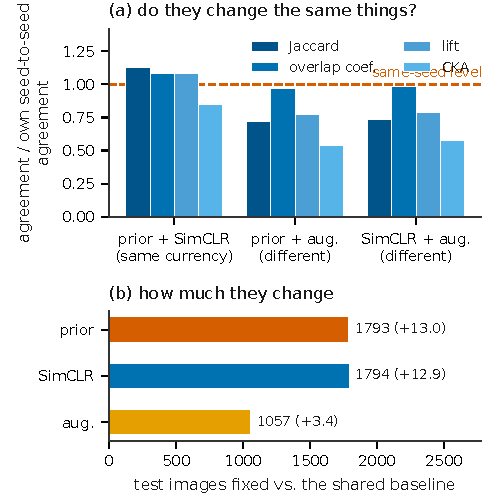
\includegraphics[width=\linewidth]{figs/currency_evidence.pdf}
\caption{Currency tested directly, not inferred from magnitudes.
All arms are ViT-tiny on CIFAR-100 at 10\% with one shared baseline, so
the only thing that varies is the fused source. \textbf{(a)} agreement
between two interventions in \emph{which} test images they fix and
\emph{which} representations they learn, each normalized by that
intervention's own seed-to-seed agreement, so $1.0$ means the two sources
differ no more than two seeds of one of them. Four measures are shown
because they do not agree on the size of the effect. \textbf{(b)} the
number of images each intervention fixes: the two same-currency sources
fix all but one the same number.}
\label{fig:currency}
\end{figure}
The prediction held on all four measures (Fig.~\ref{fig:currency}). The prior
and SimCLR fix $1793$ and $1794$ test images respectively, and their normalized
agreement on \emph{which} images is $1.13$ against $0.72$ for the prior with
augmentation; centred kernel alignment between their representations gives
$0.85$ against $0.53$. A value above one has a direct reading: for the question
of which images get fixed, it matters less whether you used a fixed spectral
target or contrastive pre-training than which seed you used. That is what a
substitute is.

Two qualifications. Augmentation fixes far fewer images ($1057$), and the
Jaccard measure penalizes a small set for being small; on the size-robust
overlap coefficient the separation shrinks to $1.08$ against $0.97$, so part of
the headline gap is a magnitude effect and only the representation-level
measure separates the pairs decisively. And this is one cell on one backbone;
it corroborates the taxonomy where the taxonomy already had its strongest
end-to-end evidence, instead of testing it somewhere new.

\emph{Takeaway.} What a source is worth depends on which currency is scarce,
not on how modern the source is: the same free prior is the most valuable
intervention we measure on an augmented ViT and the most damaging one on an
ImageNet-initialized ResNet.

%% ---------------------------------------------------------------------
\section{Validation at scale}\label{sec:scale}

Everything above could, in principle, have been a small-image regularity. We
therefore pre-registered a falsifier block and bought the two scale axes
separately: ImageNet64 (1.28M images, 1000 classes, 64\,px, 13$\times$ the
images and 5$\times$ the label space of anything else in the grid) and
ImageNet-100 at native $224$\,px with a model-scale curve (ViT-S/16, ViT-B/16,
ResNet-50, the ViTs under the standard DeiT recipe). Deviations (reduced
epochs; native-resolution transforms) apply equally to both arms of every pair.

\begin{table}[pos=htbp]
\caption{The pre-registered scale block. Every falsifier was declared
before the first run and none fired, with three qualifications kept in
view: ViT-S's $G$ landed $0.05$ below its registered band; ViT-B's
$|\Delta-G|$ of $3.12$ exceeds the registered $1.5$, on a cell whose
evaluation-ceiling limitation was also registered in advance and whose
residual is unresolvable; and
ResNet-50's $G$, registered at $-0.7$ to $-0.2$, measured $+0.19$, a $0.39$
miss across zero on a quantity that is a measured zero either way
($|\Delta - G| = 0.21$). $G$ at ImageNet64 uses the
fixed-budget evaluation (250 per class shown); ImageNet-100 the standard
full-train evaluation. Three seeds per cell; the
ImageNet-100 cells run $100$ epochs, and the text repeats both ViT pairs at
$200$, where the gains are $+4.52 \pm 0.18$ and $+6.71 \pm 0.90$.}
\label{tab:scale}
\centering\scriptsize
\setlength{\tabcolsep}{1.8pt}
\zebra{2}
\begin{tabular}{P{0.160\columnwidth}P{0.165\columnwidth}rrrP{0.145\columnwidth}}
\toprule
Cell & Registered band & $\Delta$~\up & $G$~\up & $|\Delta{-}G|$~\down & Verdict \\
\midrule
\multicolumn{6}{@{}l}{\emph{ImageNet64: 1.28M images, 1000 classes}} \\
ResNet-18 & $\Delta$: $0.0{\pm}0.5$ & $+0.04$\sem{0.08} & $+0.05$ & $0.01$ & neutral, exactly \\
MobileNetV3 & (none: in bracket) & $+1.95$\sem{0.40} & $+1.81$ & $0.14$ & consistent \\
ViT-tiny & $\Delta \geq +3$ & $+3.24$\sem{0.84} & $+2.84$ & $0.40$ & deficit persists \\
Swin-T &--& \multicolumn{3}{l}{baseline collapses at chance} & stabilized by prior \\
\midrule
\multicolumn{6}{@{}l}{\emph{ImageNet-100 @ 224\,px, DeiT recipe on ViTs}} \\
ResNet-50 & $\Delta$: $0.0{\pm}1.0$ & $-0.02$\sem{0.26} & $+0.19$ & $0.21$ & neutral at 224\,px \\
ViT-S/16 & $\Delta$: $+2..{+}8$; $G$: $12.0..12.6$ & $+13.00$\sem{0.24} & $+11.95$ & $1.05$ & above band \\
ViT-B/16 & $\Delta \geq \Delta_{\mathrm{ViT\mbox{-}S}}$ & $+26.01$\sem{2.01} & $+22.89^{*}$ & $3.12^{*}$ & grows at full data \\
\bottomrule
\rowcolor{white}\multicolumn{6}{@{}p{0.95\linewidth}@{}}{\footnotesize $^{*}$The ViT-B
aux arm evaluates at its own ceiling ($69.8$ vs.\ e2e $69.3$), a
pre-registered limitation that compresses $G$; the residual is not resolvable
against its uncertainty ($\pm 2.4$).} \\
\end{tabular}
\end{table}

Table~\ref{tab:scale} reports the block. Three conclusions.

\emph{Convolutional redundancy at sufficiency is exact and scale-stable.}
ResNet-18 at 1.28M images gains $+0.04 \pm 0.08$ end-to-end and $+0.05 \pm
0.10$ feature-side; the neutral regime measured to a hundredth of a point at
the largest data scale in the study. ResNet-50 at native $224$\,px repeats it:
the seed-paired difference on three matched seeds is $-0.02
\pm 0.26$, inside the pre-registered band ($0.0 \pm 1.0$), and the falsifier
that would have made convolutional redundancy
a low-resolution artifact ($\Delta \geq +1.5$) is ruled out.

\emph{The attention deficit is real, persistent, and grows with model scale at
full data.} ViT-tiny still gains $+3.2$ points at 1.28M images. At $224$\,px
under the standard recipe and a shared $100$-epoch budget, ViT-S/16 gains
$+13.0$ at $21.7$M parameters on a properly configured transformer, and
ViT-B/16 gains $+26.0$, twice ViT-S (the paragraphs below repeat both at a
doubled budget, where the ordering holds),
with the baseline's seed
variance three times the prior arm's. That asymmetry invites the obvious
objection, that the gain is the optimization stabilization
Sec.~\ref{abl:stab} treats as a separate property, so we settle it on the
seeds, not the standard deviation: the ViT-B baseline runs $46.5$, $39.9$ and
$43.6$, none of them near the $1\%$ chance level, so the cell does not trip the
collapse rule of Sec.~\ref{sec:stats}, and the \emph{worst} prior seed still
beats the \emph{best} baseline seed by $22$ points. Nothing here is a rescued
run. The pre-registered fork read: if the deficit is data-hunger, the bigger
model should show the larger gain. At full data it does, by 13 points. Notably,
at this budget and data scale the \emph{smaller} ViT with the prior still
outperforms the bigger one ($78.4$ vs.\ $69.3$): right-sizing plus structure
beats scale. Both are $100$-epoch numbers; at the doubled budget below, this
ordering also holds ($83.99$ against $82.02$).

\looseness=-1 That ordering was registered as a prediction across the whole envelope, not
only at full data: we recorded $\Delta_{\mathrm{ViT\text{-}B}} >
\Delta_{\mathrm{ViT\text{-}S}}$ \emph{at every fraction}, with a falsifier if
it inverted at any fraction at or above $5\%$. It inverts at $5$, $10$ and
$25\%$ (Table~\ref{tab:inenv}), so that falsifier fired and we report it (it
also inverts nominally, unresolved, at $1$ and $2\%$). We do
not read those cells as refuting the full-data result, and the reason is a
property of the arms themselves. Below $100\%$ the ImageNet-100 ViT-B baseline
never trains, flat at $4.1$--$7.1\%$ on a 100-way task across a $12.5\times$
data range, so its gain there cannot carry a claim about model scale; and the
comparator arm, ViT-S, carries baseline seed standard deviations up to $8.2$
points at exactly the fractions ($10$ and $25\%$) where it produces the
larger gain driving the inversion. The defensible claim is
the narrower one: at full data the deficit
grows with model scale, and across the low-data fractions of this population
the comparison is not determined.

\paragraph{Is the ViT-B gain an under-trained baseline?} The $+26.01$ is the
largest number in this paper and it is measured at $100$ epochs, where an
85.9M-parameter transformer on $126$k images may not have finished training. We
doubled the schedule on both arms, six seeds each.
The baseline gains $+31.98$ from the schedule alone, reaching $75.31 \pm 0.48$;
the prior arm reaches $82.02 \pm 0.76$; the gain is $+6.71 \pm 0.90$, $95\%$
confidence interval $[4.94, 8.47]$, $7.4$ standard errors from zero. About a
quarter of the headline survives a doubled schedule, so $+26.01$ is a
$100$-epoch figure and should be read with $+6.71$ beside it.

\looseness=-1 We had registered a falsifier at $\Delta \leq +6$, which would have withdrawn
the model-scale conclusion outright. The interval contains $6.0$, which sits
$0.78$ standard errors below the estimate, so the falsifier is neither fired
nor excluded and we report it as exactly that. Two facts belong beside it. The
estimate moved with seeds, $+7.79$ at three arms against two, $+7.79$ at three
against three and $+6.71$ at six against six, so a three-seed report would have
published a clearance the data do not support. And one prior-arm seed, $78.58$,
sits $4.6$ standard deviations below the other five ($82.71 \pm 0.90$); it is
not a collapse under the rule of Sec.~\ref{sec:stats} and there is no
principled reason to drop it, so it stays, and it is why this arm's uncertainty
exceeds the baseline's. Excluding it would give $+7.39 \pm 0.63$ and put the
threshold outside the interval, which is exactly why we keep it.

\paragraph{The trend at a budget where both models are trained.} The
comparison motivating that trend, $+13.00$ against $+26.01$, is made at $100$ epochs,
where the control above shows ViT-B still $+31.98$ short of where the schedule
alone takes it, so we repeated ViT-S at $200$ epochs too, six seeds per arm.
It reaches $79.47 \pm 0.16$ against $83.99 \pm 0.08$, a gain of $+4.52 \pm
0.18$, against ViT-B's $+6.71 \pm 0.90$. The ordering holds by $-2.19 \pm
0.92$, and the pre-registered falsifier, which would have withdrawn the
model-scale claim everywhere had ViT-S matched or exceeded ViT-B, did not fire.
The uncertainty is almost entirely ViT-B's (standard errors $0.48$ and $0.76$
against ViT-S's $0.16$ and $0.08$), so the ordering is clear at $2.4$ standard
errors and not tighter. We tested it expecting it to invert.

\emph{The law's predictive form survives.} Five of six pairs tie $\Delta$ to
$G$ within $1.1$ points; the sixth (ViT-B) carries a pre-registered
evaluation-ceiling limitation and an unresolvable residual. That ceiling
caveat belongs to every ImageNet-100 row, not to ViT-B alone: at these
$100\%$ cells the evaluation's labels are the cell's own, so the
$|\Delta - G|$ column is a gap read under the scope rule of
Sec.~\ref{sec:probe}, not a signed \readout{}, which is why the cells stand
here and not in the audit of Sec.~\ref{sec:lawaudit}; the ImageNet64
rows, evaluated at fixed per-class budgets, carry no ceiling. The ViT-S band,
derived from the law before the evaluation ran, was hit on its edge ($11.95$
vs.\ $12.0$--$12.6$). As an additional robustness check, the ViT-S and
ResNet-50 evaluations were independently re-run on a second machine with a
from-scratch environment; their means agree with the primary measurement to
$0.01$--$0.05$ points.

\subsection{The envelope at ImageNet scale}\label{sec:scaleenvelope}

The block above measures the right-hand end of the envelope. Because that would
leave the shape untested at scale, both ImageNet stages were also run across
fractions, on the same fixed subsets and the same reduced-epoch budget as their
$100\%$ cells (Table~\ref{tab:inenv}). This is the largest data-efficiency
envelope in the study, and it reports a registered miss before it reports
anything else.

\emph{The miss.} We registered an interior peak at $5$--$20\%$ for the
convolutional envelope. ResNet-18 instead falls from the smallest
runnable fraction, $+1.90$ at $1\%$ to zero by $10$--$15\%$, staying within
$0.2$ of zero thereafter, with no interior peak:
the falsifier fired. The cause is that we predicted in \emph{fraction} space
when the operative axis is absolute data. One percent of ImageNet64 is
$12{,}820$ images, which on every smaller population in the grid is already
past the peak. The envelope is not absent at scale; its peak sits below the
smallest fraction this dataset can express.

\emph{What the same cells then show, which we did not anticipate.} Holding
dataset, recipe, subsets and label space fixed and varying only the backbone
gives three different envelope shapes (Fig.~\ref{fig:inenv}). ResNet-18 falls
to zero and stays there; ViT-tiny and MobileNetV3 rise monotonically across the
entire measured range, ViT-tiny from $+2.14$ to $+7.75$ at $25\%$. Under the
account this is not three phenomena but one: the peak sits where the baseline
crosses the \readout{} bracket, and only ResNet-18's baseline reaches it in range
($5.5 \to 47.2$, crossing $[31.8,40.3]$ between $7$ and $15\%$), which is
exactly where its gain reaches zero ($+0.42$ at base $32.3$, $-0.01$ at base
$42.3$). Across $1$--$25\%$ neither of the others comes near the band and both
are still climbing; extend to full data and they arrive too, MobileNetV3 into
it ($32.9$) and ViT-tiny above it ($48.2$), and both gains duly fall ($+3.45
\to +1.95$ and $+7.75 \to +3.24$). One rule, three apparent shapes: the
envelope's peak is a property of where a \emph{backbone} sits on its own
\readout{} curve, not of the dataset, and this is the cleanest demonstration of
that in the paper, because the classification grid could only vary it by
changing datasets too.

\begin{figure}[pos=htbp]
\centering
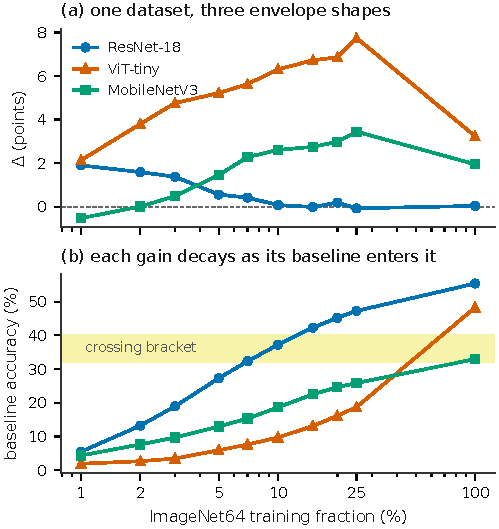
\includegraphics[width=\linewidth]{figs/inenv.pdf}
\caption{The envelope at ImageNet scale, and why its shape is a property of
the backbone. Dataset, recipe, fixed subsets and label space are held
constant; only the backbone varies. \textbf{(a)} Three backbones, three
envelope shapes: ResNet-18 falls to zero and stays there, while ViT-tiny and
MobileNetV3 climb across the whole range. \textbf{(b)} The same baselines
against the crossing bracket. Each gain decays as its own baseline enters the
band, and the three arrive at very different fractions: ResNet-18 by
$7$--$15\%$, MobileNetV3 only at $100\%$, ViT-tiny passing above it at
$100\%$, exactly where its gain falls. Three seeds per cell.}
\label{fig:inenv}
\end{figure}

\begin{table}[pos=htbp]
\caption{The envelope at ImageNet scale: $\Delta$ by fraction, three seeds
per cell, both arms sharing the reduced-epoch budget. Baseline accuracy is
given beneath each gain. ImageNet64's three backbones see identical images,
recipe and label space, so the difference in envelope \emph{shape} between
them is attributable to the backbone alone. The ImageNet-100 ViT columns
below $100\%$ are reported with a caveat, not as headline cells:
their baselines sit close to chance and carry seed standard deviations up to
$8.2$ points, so the gains there are large but poorly determined. Every
ImageNet-100 cell here uses the $100$-epoch budget; the ViT-B pair at $200$
epochs gives $+6.71$ (Sec.~\ref{sec:scale}). Best in bold and second best
underlined, per fraction within each stage; with three backbones per stage the
remaining entry is third, so no italic mark is needed.}
\label{tab:inenv}
\centering\scriptsize
\setlength{\tabcolsep}{2.2pt}
\zebra{5}
\begin{tabular}{lrrrrrr}
\toprule
& \multicolumn{3}{c}{ImageNet64, 64\,px} & \multicolumn{3}{c}{ImageNet-100, 224\,px} \\
\cmidrule(r){2-4}\cmidrule(l){5-7}
Frac. & R18 & ViT-Ti & MNetV3 & R50 & ViT-S & ViT-B \\
\midrule
1\%   & \snd{$+1.90$} & $\mathbf{+2.14}$ & $-0.52$ & $+0.54$ & $\mathbf{+2.31}$  & \snd{$+0.69$} \\
      & \tiny 5.5 & \tiny 1.9 & \tiny 4.3 & \tiny 11.5 & \tiny 7.3 & \tiny 5.3 \\
2\%   & \snd{$+1.59$} & $\mathbf{+3.80}$ & $+0.01$ & $+1.21$ & $\mathbf{+7.59}$  & \snd{$+5.11$} \\
      & \tiny 13.2 & \tiny 2.6 & \tiny 7.6 & \tiny 18.2 & \tiny 6.4 & \tiny 4.1 \\
3\%   & \snd{$+1.38$} & $\mathbf{+4.76}$ & $+0.49$ &--&--&-- \\
      & \tiny 18.9 & \tiny 3.4 & \tiny 9.7 &&& \\
5\%   & $+0.56$ & $\mathbf{+5.22}$ & \snd{$+1.46$} & $+1.84$ & $\mathbf{+14.15}$ & \snd{$+4.47$} \\
      & \tiny 27.3 & \tiny 5.9 & \tiny 12.9 & \tiny 36.5 & \tiny 7.3 & \tiny 6.1 \\
7\%   & $+0.42$ & $\mathbf{+5.63}$ & \snd{$+2.28$} &--&--&-- \\
      & \tiny 32.3 & \tiny 7.6 & \tiny 15.3 &&& \\
10\%  & $+0.08$ & $\mathbf{+6.31}$ & \snd{$+2.61$} & $+1.74$ & $\mathbf{+14.23}$ & \snd{$+2.30$} \\
      & \tiny 37.2 & \tiny 9.7 & \tiny 18.6 & \tiny 55.7 & \tiny 11.9 & \tiny 6.6 \\
15\%  & $-0.01$ & $\mathbf{+6.72}$ & \snd{$+2.75$} &--&--&-- \\
      & \tiny 42.3 & \tiny 13.1 & \tiny 22.5 &&& \\
20\%  & $+0.19$ & $\mathbf{+6.86}$ & \snd{$+2.98$} &--&--&-- \\
      & \tiny 45.2 & \tiny 16.1 & \tiny 24.6 &&& \\
25\%  & $-0.07$ & $\mathbf{+7.75}$ & \snd{$+3.45$} & $+2.30$ & $\mathbf{+30.39}$ & \snd{$+7.36$} \\
      & \tiny 47.2 & \tiny 18.7 & \tiny 25.8 & \tiny 72.5 & \tiny 23.2 & \tiny 7.1 \\
100\% & $+0.04$ & $\mathbf{+3.24}$ & \snd{$+1.95$} & $-0.02$ & \snd{$+13.00$} & $\mathbf{+26.01}$ \\
      & \tiny 55.4 & \tiny 48.2 & \tiny 32.9 & \tiny 85.9 & \tiny 65.4 & \tiny 43.3 \\
\bottomrule
\end{tabular}
\end{table}

\looseness=-1 Two further readings. The convolutional column reaches sufficiency inside the
measured range and stays there, so the neutrality result of
Table~\ref{tab:scale} is not a single point but a plateau from $10\%$ of
ImageNet64 onward. And ResNet-50 at $224$\,px is the one convolutional column
that is \emph{positive} in the low-data band ($+0.5$ to $+2.3$ from 1 to
$25\%$) before returning to neutrality at full data. We had registered $+1$ to
$+6$ across 1--5\% with a decay through $25\%$, and both halves missed: the
$1\%$ cell lands at $+0.54$, below the band, and the column rises instead of
decaying ($+1.74$ at $10\%$, $+2.30$ at $25\%$). What held is the direction and
the falsifier, which would have fired had $\Delta$ been non-positive
everywhere: convolutional gains do survive native resolution and are a
low-data, not a low-resolution, phenomenon, but we did not call their size or
their shape.

\emph{Takeaway.} Scale does not retire the prior: convolutional redundancy at
sufficiency survives 1.28M images, while attention's deficit grows with model
size, not shrinking. Filling the envelope at scale cost us a registered
prediction and returned a sharper claim in its place: which fraction the peak
sits at is a property of the backbone's position on the \readout{} curve, not of
the dataset.
